% Libraries.
\usetikzlibrary{arrows}
\usetikzlibrary{decorations.markings}

% Layers.
\pgfdeclarelayer{semiconductor}
\pgfdeclarelayer{contacts}
\pgfsetlayers{semiconductor,contacts,main}

% Styles.
\tikzstyle{semiconductor}=[fill=gray]
\tikzstyle{contact}=[fill=lightgray,opacity=0.5]

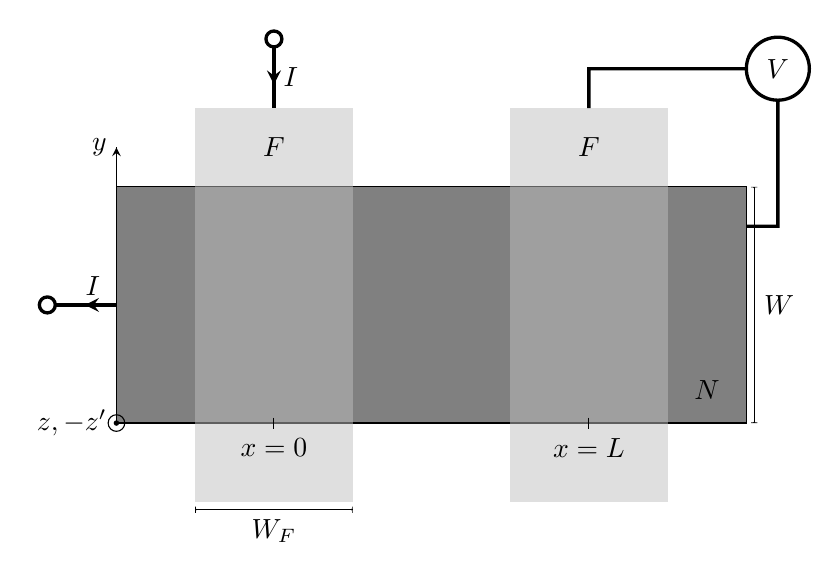
\begin{tikzpicture}
  % Guide grid.
  % \draw[step=1,gray,very thin] (0,-2) grid (10,5);

  \begin{pgfonlayer}{contacts}
    % Contacts.
    \path[contact] (1,-1) rectangle ++(2,5);
    \path[contact] (5,-1) rectangle ++(2,5);

    % Contact labels.
    \node at (2,3.5) {$F$};
    \node at (6,3.5) {$F$};

    % Contact dimensions.
    \draw[serif cm-serif cm] (1,-1.1) -- node[below] {$W_F$} ++(2,0);

    % Top current arrow.
    \begin{scope}[very thick,
      decoration={markings,
        mark=at position 0.7 with {\arrow{stealth}}}]
      \draw[o-,postaction={decorate}] (2,5) -- ++(0,-1);
    \end{scope}

    % Left current arrow.
    \begin{scope}[very thick,
      decoration={markings,
        mark=at position 0.4 with {\arrow{stealth}}}]
      \draw[-o,postaction={decorate}] (0,1.5) -- ++(-1,0);
    \end{scope}

    % Current labels.
    \draw[shift={(2,4.4)}] node[right] {$I$};
    \draw[shift={(-0.3,1.5)}] node[above] {$I$};
  \end{pgfonlayer}

  \begin{pgfonlayer}{semiconductor}
    % Semiconductor.
    \draw[semiconductor] (0,0) rectangle ++(8,3);

    % Semiconductor label.
    \node at (7.5,12pt) {$N$};

    % Semiconductor dimensions.
    \draw[serif cm-serif cm] (8.1,0) -- node[right] {$W$} ++(0,3);
  \end{pgfonlayer}

  % Voltage.
  \draw[very thick] (6,4) -- ++(0,0.5) -- ++(2,0)
    ++(0.4,0) circle [radius=0.4] node {$V$}
    ++(0,-0.4) -- ++(0,-1.6) -- ++(-0.4,0);

  % x coordinates.
  \draw[shift={(2,0)}] (0pt,2pt) -- (0pt,-2pt) node[below] {$x = 0$};
  \draw[shift={(6,0)}] (0pt,2pt) -- (0pt,-2pt) node[below] {$x = L$};

  % z-axis and z'-axis.
  \fill (0,0) circle [radius=1pt];
  \draw (0,0) circle [radius=3pt] node[left] {$z, -z'$};

  % y-axis.
  \begin{scope}[decoration={
    markings,
    mark=at position 1 with {\arrow{stealth}}}]
    \draw[postaction={decorate}] (0,0) -- (0,3.5) node[left] {$y$};
  \end{scope}
\end{tikzpicture}
